\documentclass[11pt,a4paper]{article}\usepackage[]{graphicx}\usepackage[]{color}
% maxwidth is the original width if it is less than linewidth
% otherwise use linewidth (to make sure the graphics do not exceed the margin)
\makeatletter
\def\maxwidth{ %
  \ifdim\Gin@nat@width>\linewidth
    \linewidth
  \else
    \Gin@nat@width
  \fi
}
\makeatother

\definecolor{fgcolor}{rgb}{0.345, 0.345, 0.345}
\newcommand{\hlnum}[1]{\textcolor[rgb]{0.686,0.059,0.569}{#1}}%
\newcommand{\hlstr}[1]{\textcolor[rgb]{0.192,0.494,0.8}{#1}}%
\newcommand{\hlcom}[1]{\textcolor[rgb]{0.678,0.584,0.686}{\textit{#1}}}%
\newcommand{\hlopt}[1]{\textcolor[rgb]{0,0,0}{#1}}%
\newcommand{\hlstd}[1]{\textcolor[rgb]{0.345,0.345,0.345}{#1}}%
\newcommand{\hlkwa}[1]{\textcolor[rgb]{0.161,0.373,0.58}{\textbf{#1}}}%
\newcommand{\hlkwb}[1]{\textcolor[rgb]{0.69,0.353,0.396}{#1}}%
\newcommand{\hlkwc}[1]{\textcolor[rgb]{0.333,0.667,0.333}{#1}}%
\newcommand{\hlkwd}[1]{\textcolor[rgb]{0.737,0.353,0.396}{\textbf{#1}}}%
\let\hlipl\hlkwb

\usepackage{framed}
\makeatletter
\newenvironment{kframe}{%
 \def\at@end@of@kframe{}%
 \ifinner\ifhmode%
  \def\at@end@of@kframe{\end{minipage}}%
  \begin{minipage}{\columnwidth}%
 \fi\fi%
 \def\FrameCommand##1{\hskip\@totalleftmargin \hskip-\fboxsep
 \colorbox{shadecolor}{##1}\hskip-\fboxsep
     % There is no \\@totalrightmargin, so:
     \hskip-\linewidth \hskip-\@totalleftmargin \hskip\columnwidth}%
 \MakeFramed {\advance\hsize-\width
   \@totalleftmargin\z@ \linewidth\hsize
   \@setminipage}}%
 {\par\unskip\endMakeFramed%
 \at@end@of@kframe}
\makeatother

\definecolor{shadecolor}{rgb}{.97, .97, .97}
\definecolor{messagecolor}{rgb}{0, 0, 0}
\definecolor{warningcolor}{rgb}{1, 0, 1}
\definecolor{errorcolor}{rgb}{1, 0, 0}
\newenvironment{knitrout}{}{} % an empty environment to be redefined in TeX

\usepackage{alltt}
\usepackage[top=.75in, bottom=.1in, left=.75 in, right=.75in]{geometry}
\usepackage{graphicx}
\usepackage{natbib}
\usepackage{gensymb}
%\begin{footnotesize}
%\address{1300 Centre Street \\ Boston, MA, 20131}
%\end{footnotesize}
\IfFileExists{upquote.sty}{\usepackage{upquote}}{}
\begin{document}
\bibliographystyle{..//refs/styles/besjournals.bst}
\def\labelitemi{--}
\parindent=24pt
\includegraphics[width=0.2\textwidth]{/Users/danielbuonaiuto/Desktop/arb_logo.png}
\pagenumbering{gobble}
\\\\

{Dear Dr. Pinfield-Wells,}\\
\vspace{1.5ex}

\noindent Please consider this manuscript ``Reconciling competing hypotheses regarding flower-leaf sequences in temperate forests for fundamental and global change biology" as a ''Viewpoint" article in \textit{New Phytologist}. We have corresponded with you previously about this piece through a pre-submission enquiry and received approval to submit the manuscript for full consideration.\\

\noindent A century of empirical studies suggests that flowering and leaf phenology are critical fitness components of woody plants \citep{Munguia-Rosas2011,Forrest2010}. In recent decades, research has shown that it is not only individual phenophases but also the relationship between them that determines woody plant fitness \citep{Menzel1999,Ettinger2018}. Many deciduous woody plants flower before leafing, yet sustained research efforts have yet to yield a consistant, well-supported explanation for this. These unresolved hypotheses are important now as climate change is shifting flower-leaf sequences (FLSs)---which may exacerbate fitness differences between species and reshape future ecosystems. Our ``Viewpoint" shows how progress in this area has been stalled by the current conceptual framework for FLSs; we detail a new approach that leverages continuous measures of FLSs and intra-specific and within-individual variation to rapidly advance progress.\\

\noindent \emph{What hypotheses or questions does this work address?}\\
% Nice opener!
\noindent Research suggests FLSs are under strong selection and critical to fitness. FLS variation may be an adaptation for wind-pollination \citep{Rathcke_1985}, reducing water stress \citep{Gougherty2018,Reich1984}, or early season flowering \citep{Primack1987}, but these conflicting hypotheses remain unresolved. A novel approach focusing on intra-specific FLS variation and quantitative comparisons is necessary to accurately evaluate these hypotheses.\\

\noindent \emph{How does this work advance our current understanding of plant science?}\\
\noindent We show: 1) The current framework fails to capture the inter- and intra- specific FLS variation in nature impeding robust hypothesis testing; 2) Variation provides novel insights about the function of FLSs, revealing complexities critical to advancing the hypotheses; 3) Leveraging intra-specific variation advances our understanding of FLSs.\\ % 'revealing consistencies and anomalies in support for the hypotheses' is a bit tricky to understand ... you could cut it, or replace with 'revealing complexities critical to advancing our understanding' or leave it.

\noindent \emph{Why is this work important and timely?}\\
\noindent We show that climate change is altering FLSs, but effects vary across species (0.8-4.7 days on average, Fig. \ref{fig:climchange}). Shifts could be beneficial or adverse, and predicting this outcome requires researchers to effectively evaluate the current hypotheses. Our framework is the first that can do this robustly, making it critical to fundamental and applied research.\\

\noindent The main text of this manuscript is 3370 words in length, it contains (4)5 figures. It is co-authored by I. Morales-Castilla, and E.M. Wolkovich and is not under consideration elsewhere. We hope that you will find it suitable for publication in \textit{New Phytologist}, and look forward to hearing from you.
\\Sincerely,\\\\\\\\\\

\noindent Daniel Buonaiuto\\
\pagebreak
\section*{Selected Figures:}
   \begin{figure}[ht!]
   \centering
 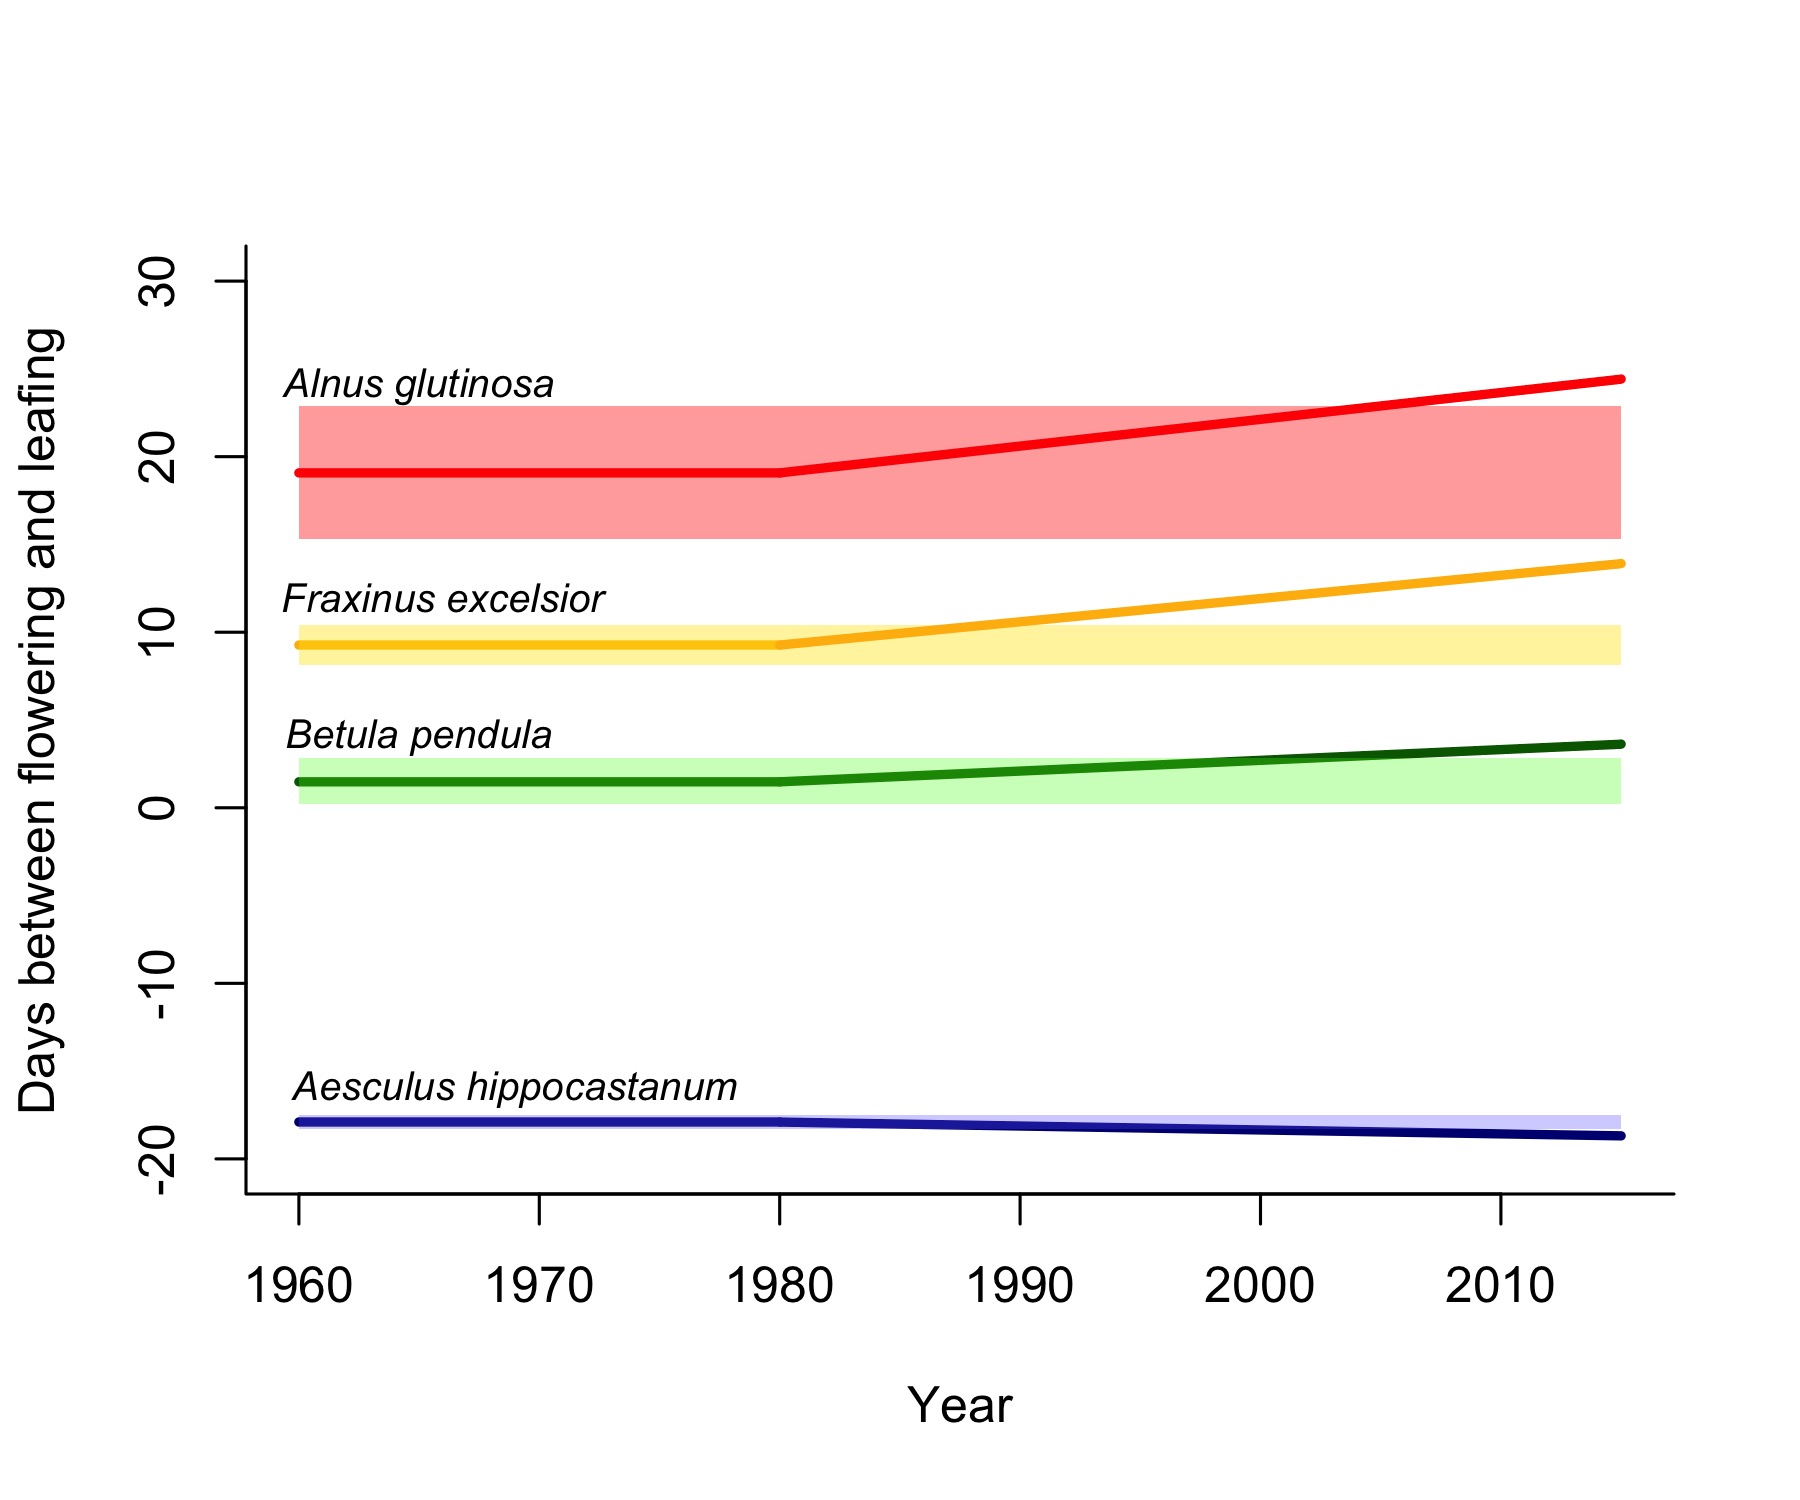
\includegraphics[width=\textwidth]{..//PEP725/FLS_climate_change.jpeg}\\
\caption{\textbf{FLSs across Europe for four tree species from 1960 to 2015 suggests climate change has generally increased the time between flowering and leafing}, but the direction and rate of change differs across species, which may exacerbate fitness differences within forest communities. To detect the effect of climate change on average FLS, we used models that allow for shifts in FLS after 1980. Lines represent the mean trend in FLS per species, and the highlighted regions indicate historic range of FLS variability (95\% credible intervals of the pre-1980 average) from the PEP725 database \citep{PEP725}.}
    \label{fig:climchange}
    \end{figure}
\newpage
\bibliography{..//refs/hyst_outline.bib}

\end{document}

